\documentclass[a4paper, notitlepage, 11pt]{article}
\usepackage{geometry}
\fontfamily{times}
\geometry{verbose,tmargin=30mm,bmargin=25mm,lmargin=25mm,rmargin=25mm}
% end configs
\usepackage{setspace,relsize}               
\usepackage{moreverb}                        
\usepackage{url}
\usepackage{hyperref}
\hypersetup{colorlinks=true,citecolor=blue}
\usepackage{subfigure}
\usepackage{amsmath}
\usepackage{mathtools} 
\usepackage{amsthm}
\usepackage{amssymb}
\usepackage{indentfirst}
\usepackage{todonotes}
\usepackage[authoryear,round]{natbib}
\bibliographystyle{apalike}
\usepackage[pdftex]{lscape}
\usepackage[utf8]{inputenc}

% Title Page
\title{\vspace{-9ex}\centering \bf On the propriety of power priors}
\author{
% Luiz Max de Carvalho\\
% Program for Scientific Computing (PROCC), Oswaldo Cruz Foundation. \\
}
\DeclareMathOperator*{\argmin}{arg\,min}
\DeclareMathOperator*{\argmax}{arg\,max}
\newtheorem{theorem}{Theorem}[]
\newtheorem{proposition}{Proposition}[]
\newtheorem{remark}{Remark}[]
\setcounter{theorem}{0} % assign desired value to theorem counter
\begin{document}
\maketitle

% \begin{abstract}
% 
% Key-words: ;; ; ; . 
% \end{abstract}

\section{Background}

\begin{itemize}
 \item Power priors are cool. [bunch of citations for propriety of GLM, Cox model, exponential family, etc];
 \item In this paper we explore the situation where the initial prior $\pi$ is proper;
 \item We also explore ways of approximating the normalising constant $c(a_0)$ for models where it cannot be written in closed-form. 
\end{itemize}

\textbf{Definition}
The data $D_0 = \{ d_{01}, \ldots, d_{0N_0} \} \in \mathcal{X} \subseteq \mathbb{R}^p$ are assumed independent and identically distributed  and the parameter $\theta \in \Theta \subseteq \mathbb{R}^q$ and $a_0 \geq 0$.
\begin{equation}
\label{eq:power_prior}
 p(\theta \mid D_0, a_0) \propto L(D_0 \mid \theta)^{a_0}\pi(\theta).
\end{equation}

\section{Results}

We want to show under which conditions
\[\int_{\Theta} L( D_0 \mid \theta)^{a_0}\pi(\theta) d\theta <\infty.\]
\begin{theorem}
\label{thm:integrability}
 Assume $\int_{\mathcal{X}} L( x \mid \theta)dx < \infty$.
 Denote $f_{a_0}(D_0;\theta) : = L( D_0 \mid \theta)^{a_0}\pi(\theta)$.
 Then for $a_0 > 0$, $\int_{\Theta} f_{a_0}(D_0;\theta) d\theta <\infty$.
\end{theorem}
\begin{proof}
First, note that for $0 < a_0 \leq 1$, the function $g(x) = x^{a_0}$ is concave.
Then, by Jensen's inequality and the finiteness of $L( D_0 \mid \theta)$ for all of its arguments we have
\[ \int_{\Theta} f_{a_0}(D_0; \theta) d\theta \leq \left[ \int_{\Theta} L(D_0 \mid\theta)\pi(\theta)d\theta \right]^{a_0} < \infty. \]
Rewrite $f_{a_0}(D_0; \theta) = L(D_0\mid\theta)^{a_0 -1} L(D_0\mid\theta)\pi(\theta)$.
If $1 \leq a_0 \leq 2$, we have the Jensen's inequality case above, since we know that $L(D_0\mid\theta)\pi(\theta)$ is normalisable.
Similarly, if $2 \leq a_0 \leq 3$, we can write 
\[  f_{a_0}(D_0; \theta) = L(D_0\mid\theta)^{a_0-p} L(D_0\mid\theta)^p\pi(\theta), \]
with $1 \leq p \leq 2$, again falling into the same case, since we know that $L(D_0\mid\theta)^{p}\pi(\theta)$ is normalisable.
We can then show that for any $n \geq 1 \in \mathbb{N}$, $\int_{\Theta}f_{a_0}( D_0 ; \theta)d\theta < \infty$ for  $n-1 \leq a_0 \leq n$.
The base case for $1 \leq n \leq 3$ is established.
Now suppose the hypothesis holds for $n \geq 3$.
For $n + 1$ we have for $ n \leq  a_0 \leq n + 1$ and $n-1 \leq p_n \leq n$:
\begin{align*}
 \int_{\Theta} L(D_0\mid\theta)^{a_0-p_n} L(D_0\mid\theta)^{p_n}\pi(\theta)d\theta < \infty, \\
\end{align*}
because $0 \leq a_0 - p_n \leq 1$ and $L(D_0\mid\theta)^{p_n}\pi(\theta)$ is proper by hypothesis.
\end{proof}
\begin{remark}
 The power prior on multiple (independent) historical data sets is also a proper density.
\end{remark}
\begin{proof}
 Recall that the power prior on multiple historical data sets is of the form~[Eq. 2.9]\citep{Ibrahim2015}:
 \[ \pi(\theta \mid \boldsymbol D, \boldsymbol a_0) \propto \prod_{k=1}^K L(\theta \mid D_k)^{a_{0k}} \pi_0(\theta). \]
Assume, without loss of generality, that $L(\theta \mid  D_k)^{a_{0k}} > 1$ for all $\theta$ and let $m := \max(\boldsymbol a_0)$ with $\boldsymbol a_0 := \{ a_{01}, a_{02}, \ldots, a_{0K}\}$.
Then $\pi(\theta \mid \boldsymbol D, a_0)$ is bounded above by 
\[  g(\theta) :=  \prod_{k=1}^K L(\theta \mid D_k)^{m} \pi_0(\theta) =  \left[ \prod_{k=1}^K L(\theta \mid D_k) \right]^m  \pi_0(\theta) = L(\theta \mid \boldsymbol D)^m \pi_0(\theta), \]
which is normalisable following Theorem~\ref{thm:integrability}.
To relax the assumption made in the beginning, notice that this construction also bounds the case $ 0 \leq  L(\theta \mid  D_k)^{a_{0k}} \leq 1$ (for some $k$) above.
\end{proof}

\subsection{Properties of the normalising constant $c(a_0)$}

\begin{remark}
\label{rmk:convex_norm_constant}
 The normalising constant is a convex function of $a_0$.
\end{remark}
\begin{proof}
Define the normalising constant as a function $c : [0, \infty) \to (0, \infty)$,
\begin{equation}
 \label{eq:normconst}
 c(a_0) := \int_{\Theta} L(D_0\mid\theta)^{a_0} \pi(\theta)d\theta,
\end{equation}
which is positive and continuous on its domain.
The first and second derivatives are
\begin{align}
\label{eq:derivative_ca0}
c^\prime(a_0) &= \int_{\Theta} L(D_0\mid\theta)^{a_0} \pi(\theta) \log L(D_0\mid\theta) d\theta, \\
c^{\prime\prime}(a_0) &= \int_{\Theta} L(D_0\mid\theta)^{a_0} \pi(\theta) [\log L(D_0\mid\theta)]^2 d\theta,
\end{align}
and the integrals always exist (see Proposition~\ref{prop:c_is_C2} in Appendix~\ref{sec:further_proofs}). %% LM: to see why, recall that L(D|t) bounds log L(D|t) above.
From this we conclude that $c$ is (strictly) convex and $c^\prime$ is monotonic, because $c^{\prime\prime}$ is always positive.
\end{proof}
For the goals of this paper, it would be useful to know more about the shape of $c(a_0)$, more specifically if and when its derivatives change signs.
Let us first study an upper bound for $c^\prime(a_0)$.
By a straight-forward application of the Cauchy-Schwarz inequality, we also know that $c^{\prime\prime}(a_0) \geq c^\prime(a_0)$.
Now, to derive a lower bound on $c^\prime(a_0)$, consider the inequality $ 1- 1/x \leq \log(x)$, $x >0$, which suggests
\begin{equation*}
 \label{eq:c_a0_deriv_lb}
 c^\prime(a_0) \geq c(a_0) - \int_{\Theta} L(D_0\mid\theta)^{a_0-1} \pi(\theta) d\theta.
\end{equation*}


\subsubsection{Exponential family}

Suppose $L(D_0 \mid \theta)$ is in the exponential family:
\begin{equation}
 L(D_0 \mid \theta) = \boldsymbol h(D_0) \exp \left( \eta(\theta)^T \left(\sum_{i=1}^{N_0} T(d_{0i}) \right) - N_0 A(\theta) \right),
\end{equation}
where $\boldsymbol h(D_0) = \prod_{i = 1}^{N_0} h(d_{0i})$.
Thus we have
\begin{align}
 c(a_0) &=  \int_{\boldsymbol\Theta} \left[ \boldsymbol h(D_0) \exp \left( \eta(\theta)^T \left(\sum_{i=1}^{N_0} T(d_{0i}) \right) - N_0 A(\theta) \right) \right]^{a_0}\pi(\theta) d\theta, \\
  \label{eq:expo_family_const}
 &= \boldsymbol h(D_0)^{a_0}\int_{\boldsymbol\Theta} \exp \left( \eta(\theta)^T \left(a_0 \sum_{i=1}^{N_0} T(d_{0i}) \right) \right) \exp\left(- a_0N_0 A(\theta) \right) \pi(\theta) d\theta.
\end{align}
The derivative evaluates to 
\begin{equation}
\label{eq:expo_family_deriv_general}
 c^\prime(a_0) = \log(\boldsymbol h(D_0)) + \int_{\boldsymbol\Theta} \eta(\theta)^T \left(a_0 \sum_{i=1}^{N_0} T(d_{0i}) \right) f_{a_0}(D_0; \theta) d\theta -  a_0N_0\int_{\boldsymbol\Theta} f_{a_0}(D_0; \theta)  A(\theta) d\theta,
\end{equation}
where $f_{a_0}(D_0; \theta) := L(D_0 \mid \theta)^{a_0}\pi(\theta)$.

If we choose $\pi(\theta)$ to be conjugate to $L(D_0 \mid \theta)$~\citep{Diaconis1979}, i.e.
\begin{equation}
 \label{eq:conj_exp_family}
 \pi(\theta \mid \tau, n_0) = H(\tau, n_0) \exp\{ \tau^T\eta(\theta) - n_0A(\theta) \},
\end{equation}
we have 
\begin{align}
 \label{eq:expo_family_const_conj}
%  c(a_0) &= \boldsymbol h(D_0)^{a_0} H(\tau, n_0) \int_{\boldsymbol\Theta} \exp \left( \eta(\theta)^T \left(a_0 \sum_{i=1}^{N_0} T(d_{0i}) \right) -a_0N_0 A(\theta) \right) \exp\{  \eta(\theta)  \tau^T - n_0A(\theta) \} d\theta,\\
 c(a_0) &= \boldsymbol h(D_0)^{a_0} H(\tau, n_0) \int_{\boldsymbol\Theta}  \exp \left[ \eta(\theta)^T \left( \tau + a_0\sum_{i=1}^{N_0} T(d_{0i}) \right) -(n_0  + a_0N_0) A(\theta) \right] d\theta
\end{align}

\subsection{Examples}
\subsubsection{Gaussian}

Suppose one has $N_0$ historical observations $y_{i0} \in \mathbb{R}, i = 1, \ldots, N_0$.
Here we will choose a Normal-gamma conjugate model:
\begin{align*}
 \tau &\sim \text{Gamma}(\alpha_0, \beta_0),\\
 \mu &\sim \text{Normal}(\mu_0, \kappa_0\tau ),\\
 y_{0i} \mid \mu, \tau &\sim \text{Normal}(\mu, \tau),
\end{align*}
where the normal distribution is parametrised in terms of mean and precision (see below for a different parametrisation).
The posterior distribution is again a normal-gamma distribution and the normalising constant is
\begin{align}
 \label{eq:cA0_gaussian}
 c(a_0) &= \frac{\Gamma(\alpha_n)}{\Gamma(\alpha_0)}\frac{\beta_0^{\alpha_0}}{\beta_n^{\alpha_n}} \left(\frac{\kappa_0}{\kappa_n} \right)^2 (2\pi)^{-N_0 a_0/2},\\
 \nonumber
 \alpha_n &= \alpha_0 + \frac{1}{2}a_0N_0 \\
 \nonumber
 \kappa_n &= \kappa_0 + a_0N_0 \\
 \nonumber
 \beta_n  &= \beta_0 + \frac{1}{2}\left( a_0\sum_{i=1}^{N_0}(y_{0i}-\bar{y})^2 + \left(\kappa_0 a_0 N_0 (\bar{y}-\mu_0)^2\right)/\kappa_n \right),
\end{align}
with $\bar{y} = \sum_{i=1}^{N_0} y_{0i}/N_0$.

\subsubsection{Linear regression with a normal inverse-Gamma prior}

Suppose $\boldsymbol X_0$ is a $N_0 \times P$ full-rank matrix of predictors and $\boldsymbol y_0 = \{y_{01}, \ldots, y_{0N_0} \}$ is a vector of observations.
For illustrative purposes, we will employ a mean and variance parametrisation, which naturally leads to a normal inverse-gamma conjugate prior.
The model is 
\begin{align*}
 \sigma^2 &\sim \text{Inverse-gamma}(\alpha_0, \beta_0),\\
 \epsilon_i \mid \sigma^2  &\sim \text{Normal}(0, \sigma^2), \\
 \beta \mid \sigma^2 &\sim \text{Normal}(\boldsymbol \mu_0, \sigma^2\boldsymbol\Lambda_0^{-1}),\\
 y_{0i} &= \boldsymbol X_{0i}^\top \boldsymbol\beta + \epsilon_i, \\
\end{align*} 
where $\boldsymbol\beta$ is a $ 1 \times P$ vector of coefficients.
The posterior is again a normal inverse gamma and thus
\begin{align}
 \label{eq:cA0_regression}
c(a_0) &= \sqrt{\frac{|\boldsymbol\Lambda_n|}{|\boldsymbol\Lambda_0^{-1}|}} \frac{\beta_0^{\alpha_0}}{\beta_n^{\alpha_n}}\frac{\Gamma(\alpha_0)}{\Gamma(\alpha_n)}  (2\pi)^{-N_0 a_0/2},\\
\nonumber
\boldsymbol\Lambda_n &= \boldsymbol X_{\star}^\top\boldsymbol X_{\star} + \boldsymbol \Lambda_0^{-1}, \\
\nonumber
\boldsymbol\mu_n &= \boldsymbol\Lambda_n^{-1}\left(\boldsymbol\Lambda_0^{-1}\boldsymbol\mu_0 + \boldsymbol X_{\star}^\top\boldsymbol y_{\star} \right)  \\
\nonumber
\alpha_n &= \alpha_0 + \frac{1}{2}a_0N_0,\\
\nonumber
\beta_n &= \beta_0 + \frac{1}{2}\left( \boldsymbol y_{\star}^\top \boldsymbol y_{\star} + \boldsymbol \mu_0^\top \boldsymbol \Lambda_0^{-1} \boldsymbol \mu_0 - \boldsymbol\mu_n^\top \boldsymbol \Lambda_n \boldsymbol \mu_n  \right),
\end{align}
where $\boldsymbol X_{\star} = \sqrt{a_0} \boldsymbol X_0$ and $\boldsymbol y_{\star} = \sqrt{a_0} \boldsymbol y_0$, and $|A|$ denotes the determinant of $A$.

\subsubsection{Bernoulli}

The historical data consist of $N_0$ Bernoulli trials $x_{0i} \in \{0,1\}$.
Suppose there were $y_0 = \sum_{i=1}^{N_0}x_{0i}$ successes.
The model reads
\begin{align*}
 \theta &\sim \text{Beta}(c, d), \\
 x_{0i} \mid \theta &\sim \text{Bernoulli}(\theta).
\end{align*}
This leads to a Beta posterior distribution for $\theta$,
\begin{equation}
 \label{eq:bernoulli_posterior}
 p(\theta | N_0, y_0, a_0) \propto \theta ^{a_0 y_0 + c - 1} (1-\theta)^{a_0 (N_0 -y_0) + d - 1},
\end{equation}
and hence~\citep{Neuenschwander2009}:
\begin{equation}
 \label{eq:cA0_bernoulli}
 c(a_0) = \frac{\mathcal{B}(a_0 y_0 + c, a_0 (N_0 -y_0) + d)}{\mathcal{B}(c, d)},
\end{equation}
where $\mathcal{B}(w, z) = \frac{\Gamma(w)\Gamma(z)}{\Gamma(w + z)}$.

% \subsubsection{Binomial}
% The binomial variant is quite similar to the Bernoulli model, with the model

\subsubsection{Gamma}

The historical data consist of $N_0$ observations $\boldsymbol y_0 =\{y_{01}, \ldots , y_{0N_0}\}$, $y_{0i} > 0$.
And the model is
\begin{align*}
 \alpha &\sim \text{Gamma}(\eta_\alpha, \nu_\alpha), \\
 \beta &\sim \text{Gamma}(\eta_\beta, \nu_\beta), \\
 y_{0i} \mid \alpha, \beta &\sim \text{Gamma}(\alpha, \beta).
\end{align*}
The posterior distribution is 
\begin{equation}
 \label{eq:posterior_gamma}
 p(\alpha, \beta | \boldsymbol y_{0}, a_0) \propto \frac{\beta^{a_0N_0\alpha}}{\Gamma(\alpha)^{a_0N_0}} \boldsymbol p^{a_0(\alpha-1)} \exp(-a_0\boldsymbol s\beta) \times  \alpha^{\eta_\alpha -1} \exp(-\nu_\alpha \alpha) \times \beta^{\eta_\beta -1} \exp(-\nu_\beta \beta),
\end{equation}
where $\boldsymbol p := \prod_{i =1}^{N_0} y_{0i}$ and $\boldsymbol s := \sum_{i =1}^{N_0} y_{0i}$.
Noticing that the full conditional distribution of $\beta$ is (the kernel of) a Gamma distribution leads to
\begin{align}
 \label{eq:cA0_gamma}
 c(a_0) = \frac{\nu_\alpha^{\eta_\alpha}\nu_\beta^{\eta_\beta}}{\Gamma(\eta_\alpha)\Gamma(\eta_\beta)} \frac{1}{\boldsymbol p^{a_0} } \times \int_0^\infty \frac{\Gamma(a_0N_0\alpha + \eta_\beta)}{\left( a_0\boldsymbol s + \nu_\beta \right)^{a_0N_0\alpha + \eta_\beta}} \frac{\alpha^{\eta_\alpha -1} \exp(- ( \nu_\alpha - a_0 \log \boldsymbol p) \alpha)}{\Gamma(\alpha)^{a_0 N_0}} d\alpha.
\end{align}
Whilst the expression in~(\ref{eq:cA0_gamma}) cannot be obtained in closed-form, it can be approximated \textit{via} quadrature.


\subsubsection{Inverse Gaussian}

The historical data consist of $N_0$ observations $\boldsymbol y_0 =\{y_{01}, \ldots , y_{0N_0}\}$, $y_{0i} > 0$.
The model is
\begin{align*}
 \mu & \sim~\text{Gamma}(\alpha_\mu, \beta_\mu),\\
 \lambda & \sim~\text{Gamma}(\alpha_\lambda, \beta_\lambda),\\
 y_{0i} \mid \mu, \lambda &\sim~\text{Inverse-Gaussian}(\mu, \lambda).
\end{align*}

The posterior distribution is
\begin{align}
  \nonumber
 p(\mu, \lambda | \boldsymbol y_0, a_0) &\propto \left(\frac{\lambda}{2\pi}\right)^{\frac{1}{2}a_0N_0} \boldsymbol p^{-\frac{3}{2} a_0} \exp\left( -a_0\left[ \frac{\boldsymbol s}{2\mu^2} -\frac{N_0}{\mu} + \frac{\boldsymbol s^\prime}{2} \right]\lambda\right) \times \\
 \label{eq:posterior_invGauss}
 &\mu^{\alpha_\mu-1}\exp(-\beta_\mu \mu) \lambda^{\alpha_\lambda -1} \exp(-\beta_\lambda  \lambda),
\end{align}
where  $\boldsymbol p := \prod_{i =1}^{N_0} y_{0i}$,  $\boldsymbol s := \sum_{i =1}^{N_0} y_{0i}$ and $\boldsymbol s^\prime := \sum_{i =1}^{N_0} \frac{1}{y_{0i}}$.
Similar to the Gamma case, one can marginalise over $\lambda$ by noticing its full conditional distribution is a Gamma distribution (see Appendix):
\begin{align}
 \nonumber
 c(a_0) &= \frac{\beta_\mu^{\alpha_\mu}\beta_\lambda^{\alpha_\lambda} }{\Gamma(\alpha_\mu)\Gamma(\alpha_\lambda)} \times (2\pi)^{-\frac{1}{2}a_0N_0} \boldsymbol p^{-\frac{3}{2} a_0} \Gamma\left( \frac{a_0N_0 + 2\alpha_\lambda}{2} \right) \times \\
 \label{eq:cA0_invGaussian}
 & \int_0^\infty \left( \frac{a_0\boldsymbol s}{2\mu^2} -\frac{a_0N_0}{\mu} + \frac{ a_0 \boldsymbol s^\prime}{2} + \beta_\lambda \right)^{-\frac{a_0N_0 + 2\alpha_\lambda}{2}} \mu^{\alpha_\mu-1}\exp(-\beta_\mu \mu) d\mu.
\end{align}
Again, while the integral in~(\ref{eq:cA0_invGaussian}) is not known in closed-form, it can be approximated~\textit{via} quadrature.


\subsubsection{Poisson}

Suppose the historical data consists of $N_0$ observations $y_{0i} \in \{0, 1, \ldots \}$.
The model is 
\begin{align*}
 \lambda &\sim \text{Gamma}(\alpha_0, \beta_0),\\
 y_{0i} \mid \lambda &\sim \text{Poisson}(\lambda).
\end{align*}
The posterior distribution is 
\begin{equation}
 p(\lambda \mid \boldsymbol y_0) \propto \frac{1}{\boldsymbol {p^\prime}^{a_0} } \lambda^{a_0\boldsymbol s} \exp(-a_0 N_0 \lambda) \times \lambda^{\alpha_0-1} \exp(-\beta_0\lambda),
\end{equation}
where $\boldsymbol s := \sum_{i=0}^{N_0} y_{0i}$ and $\boldsymbol p^\prime := \prod_{i = 0}^{N_0} y_{0i}!$, leading to
\begin{equation}
 \label{eq:cA0_poisson}
 c(a_0) = \frac{\beta_0^{\alpha_0}}{\Gamma(\alpha_0)}\frac{1}{\boldsymbol {p^\prime}^{a_0} } \frac{\Gamma(a_0\boldsymbol s + \alpha_0)}{\left( a_0N_0 + \beta_0 \right)^{a_0\boldsymbol s + \alpha_0} }.
\end{equation}


\subsection{Efficiently computing $c(a_0)$}

For many models, $c(a_0)$ is not known in closed form, and hence must be approximated if we wish to compute it.
An example where this would be important is when we need to normalise the power prior for use within a Markov chain Monte Carlo (MCMC) procedure.

Here we take the following approach to approximating $c(a_0)$: first, define a grid of values $\boldsymbol a^{\text{est}} = \{ a^{\text{est}}_1, \ldots, a^{\text{est}}_J \}$ for a typically modest number $J$.
Using a marginal likelihood approximation method (see below), compute an estimate of $c(a_0)$ for each point in $\boldsymbol a^{\text{est}}$, obtaining a set of estimates.
Consider an approximating function $g_{\boldsymbol\xi} : \mathbb{R}^+ \to \mathbb{R}^+$, indexed by a set of parameters $\boldsymbol\xi$.
For instance, $g_{\boldsymbol\xi}$ could be a linear model, a generalised additive model (GAM) or a Gaussian process.
We can then use  $\boldsymbol a^{\text{est}}$ and $\hat{\boldsymbol c}$ as data to learn about $\boldsymbol\xi$.
Once we obtain an estimate  $\hat{\boldsymbol \xi}$, $c(\cdot)$ can be approximated at any point $z$ by the prediction $g_{\hat{\boldsymbol \xi}}(z)$.

In order to simplify implementation, in our applications we found it useful to create a grid of size $K \gg J$, $\boldsymbol a^{\text{pred}} = \{ a^{\text{pred}}_1, \ldots, a^{\text{pred}}_K \}$, and then compute the predictions $\boldsymbol g^{\text{pred}} := g_{\hat{\boldsymbol \xi}}( \boldsymbol a^{\text{pred}} )$.
We can then use this dictionary of values to obtain an approximate value of $c(a_0)$ by simple interpolation.
This approach allows one to evaluate several approximating functions without having to implement each one separately.

A key insight is that $c(a_0)$ is convex, so we need only to make sure our grid covers the region where its derivative changes signs when designing both $\boldsymbol a^{\text{est}}$ and $\boldsymbol a^{\text{pred}}$.

A caveat of this grid approach is that the maximum end point needs to be chosen in advance, effectively bounding the space of $a_0$ considered. 
For many applications, interest usually lies with $a_0 \in [0, 1]$, and in applications where one is interested in $a_0 > 1$, one usually has a good idea of the range of reasonable of values, since this information is also useful in specifying the prior $\pi(a_0)$.
In fact, prior information can be used to set the maximum grid value: let $p$ be a fixed probability and then set the maximum grid value $M$ such that
\[ \int_0^M \pi(a) da = p. \]
One can pick $p = 0.9999$, for instance so as to have a high chance of not sampling any values outside the grid.

\textbf{Effect of discretising the approximating function}.
In order to evaluate the effect of discretisation of $g_{\boldsymbol\xi}$ on inferences, we evaluated the effect of varying the prediction grid size $K$.
For three examples where we know the truth, namely the Gaussian and Bernoulli distributions and a linear regression with a normal inverse-Gamma prior, we compared estimates of parameters -- including $a_0$ -- and marginal likelihoods obtained by using the true $c(a_0)$ and the discretised $g_{\boldsymbol\xi}$ with $K =  50, 100, 1000,~\text{and}\: 10, 000$.
For prediction, we use a simple, linear grid, with end points $a^{\text{pred}}_1 = 0$ and $a^{\text{pred}}_K = 10$.
For all experiments we fixed the estimation grid size at $J = 10$ with the same endpoints as the prediction grid $a^{\text{est}}_1 = 0$, $a^{\text{est}}_K = 10$, but placing most ($J-3 = 7$) points on the $[0, 1]$ interval.

\textbf{Marginal likelihood estimation}.
We employed  bridge sampling to compute marginal likelihoods implemented in the R package~\textbf{bridgesampling}~\citep{Gronau2017}.
We used HMC as before, with four independent chains of $2000$ iterations each, removing half of each chain as burn-in/warm-up, resulting in $4000$ samples being kept.


% \section*{Comments}
% \begin{itemize}
%  \item  Q: Why is Remark~\ref{rmk:convex_norm_constant} -- and other results in the same spirit -- useful? 
%  
%  A: because for many models we will have NO IDEA what $c(a_0)$ is but may still want to normalise the power prior and hence will have to try and approximate it. 
%  Computing $c(a_0)$ \textit{via} traditional normalising constant estimation for arbitrary values of $a_0$ within an MCMC run is impratical.
%  Hence, we would need curve estimation/approximation methods to get quick and reasonably accurate estimates of the~\textit{function} $c(a_0)$, and knowing that it is convex or monotonic or whatever would help restrict the search space.
% \end{itemize}

\section*{TODO:}
\begin{itemize}
 \item check proofs;
\end{itemize}

% \section{Roadmap}
% The idea is to review and justify power priors for general regression models.
% Since the integral of~(\ref{eq:power_prior}) with respect to $\theta$ is quite complicated, it is nice and reassuring to know that it is computable, even we don't quite know how to compute it.
% So we need to
% \begin{itemize}
%  \item Review the necessary literature;
%  \item Write down a couple examples of interesting regression models: random effects and Cox model with right-censoring (cure rate/ promotion time model);
%  \item See if we can prove a few more interesting things about these models;
%  \item Show our general results and argue that they provide justification for general use of power priors: they can be normalised, even if sometimes it is very hard to do so.
%  \item Find and curate ``classic'' data sets and write some Stan code to fit the models above to them;
% \end{itemize}
% As I understand it currently, the paper would have review-y feel to it: review what has been done for regression models and then add some of new stuff we've figured out.

\section{Questions}

\begin{enumerate}
%  \item Is it not the case that when employing an unormalised power prior, we can't compute marginal likelihoods\footnote{What I mean to say here is that marginal likelihoods don't make any sense unless the prior is properly normalised.}? Does that matter in practice? LM: Yeah, you need a properly normalised prior.
%  \item Should we be pursuing ways of computing $c(a_0) := \int_{\boldsymbol \Theta} p(t \mid D, a_0)dt$ for general models? LM: YES!
\item \textbf{The shape of $c(a_0)$}: From both a theoretical and practical point of view, it'd be nice to know when $c(a_0)$ is non-monotonic like for the Gaussian case [and a very special choice of hyperparameters] and when it's just a straight line, as for most models I've tested. 
Appendix~\ref{sec:ca0_norm_deriv} contains some rudimentary analysis for the Gaussian case...
\item \textbf{Exponential family}: it could be potentially fruitful to explore the results in Eq.~\ref{eq:expo_family_const} a bit more and maybe help answer the question above; under which conditions will a likelihood in the exponential family lead to a monotonic (and hence linear since we know it's definitely convex) $c(a_0)$?
\item \textbf{Sensitivity to $a_0$}: (i) is this important? (ii)  how to define sensitivity? one thing to look at is variance reduction as $a_0 \to \infty$...
At any rate, we know empirically that for some models (e.g. logistic regression) including the normalising constant is of utmost importance, whereas for others (e.g. Bernoulli), it doesn't seem to matter much.
\textbf{Important:} When I say ``matters'' (or not), I'm talking about the effect on estimates of actual parameters, like regression coefficients or success probability.
Including $c(a_0)$ always makes a HUGE difference for ``estimates'' of $a_0$, obviously.
\item \textbf{Situations with $a_0 > 1$} Should we pursue this? It seems to me we should at least consider it, since we show that the power prior is proper for $a_0 > 1$ also.
\end{enumerate}


\section*{Acknowledgements}

LMC would like to thank Leo Bastos (PROCC/Fiocruz) for helpful discussions and Dr. Beat Neuenschwander for clarifications regarding his paper.
This study was financed in part by the Coordenação de Aperfeiçoamento de Pessoal de Nível Superior - Brasil (CAPES) Finance Code 001.
LMC is supported by a postodoctoral fellowship from CAPES.

\bibliography{../biblio/power_prior}

\appendix

\section{Additional results}
\label{sec:further_proofs}

\begin{proposition}
\label{prop:c_is_C2}
The first and second derivatives of $c(a_0)$ always exist, i.e., $c \in \mathcal{C}^2$. 
\end{proposition}
\begin{proof}
Here we will assume that $L(D_0 \mid \theta) > 0\: \forall \theta \in \Theta$.
Let $f(\theta) = L(D_0 \mid \theta)^{a_0}\pi(\theta)$.
To see that
\[c^\prime(a_0) = \int_{\Theta} L(D_0\mid\theta)^{a_0} \pi(\theta) \log L(D_0\mid\theta) d\theta < \infty, \]
make $ X = L( D_0 \mid \theta)$ and  apply Jensen's inequality to get $E_f[\log(X)] \leq \log\left(E_f[X]\right)$, then apply Theorem~\ref{thm:integrability}.
Now, to show that 
\[ c^{\prime\prime}(a_0) = \int_{\Theta} L(D_0\mid\theta)^{a_0} \pi(\theta) [\log L(D_0\mid\theta)]^2 d\theta < \infty, \]
we will first assume that $L(D_0 \mid \theta) < 1 \: \forall\: \theta \in \Theta$, because if $L(D_0 \mid \theta) > 1$, the integral is bounded above by $c(a_0 + 2)$ and hence is clearly finite.
For $0 < x \leq 1$, the usual bounds on $\log(x)$ can be manipulated to get 
% $$ (x-1)\log(x) \leq \log(x)\log(x) \leq \left(1 - \frac{1}{x}\right)\log(x) \leq - \frac{\log(x)}{x} $$
$$ (x-1)\log(x) \leq \log(x)\log(x) \leq - \frac{\log(x)}{x} $$
% From this we conclude that 
% \[ E_f[X\log(X)] - E[\log(X)] \leq E_f[\log(X)\log(X)] \leq - E_f[\log(X)/X], \]
Hence all that remains is to show that $ - \infty < E_f[\log(X)/X]$.
Again, we can manipulate the bounds on $\log(x)$ to get $1/x - 1/x^2 \leq \log(x)/x$, so we need to show that $E[1/X^2] < \infty$.
This holds for $a_0 \geq 2$, but we shall try to show the result in general.
% \[ E[1/X^2] = \int_{\Theta} L(D_0\mid\theta)^{a_0-2}\pi(\theta)  d\theta\]
% For $a_0 = 0$,
% \[ E[1/X^2] = \int_{\Theta} \frac{\pi(\theta)}{L(D_0\mid\theta)^2}  d\theta\]
Define the random variable $Y = \left[L(D_0 \mid \theta)\right]^2$, let $G$ be the push-forward measure on $Y$ induced by $\Pi_\theta$, and let $g(y)$ be its density.
Then we can write 
\[ f_Y(y) = L(D_0\mid\theta)^{a_0}\pi(\theta) = y^{a_0/2} g(y). \]
Notice that asking that $E[1/X^2] < \infty$ is equivalent to asking that $E[Y^{-1}] < \infty$.
Corollary 2.1 of ~\cite{Piegorsch1985} states that if $Y$ is a positive random variable and $f_Y^\prime(0)$ exists and is finite, then $E[Y^{-1}] < \infty$.
Since 
\[ f_Y^\prime(y) = y^{(a_0-2)/2} \left(\frac{a_0}{2}g(y) + yg^\prime(y) \right),\]
we have $f_Y^\prime(0) = 0$ and hence 
% Theorem says that if $Y$ is a positive random variable and for some $\alpha > 0$
% \[ \lim_{y \to 0} \frac{f_Y(y)}{y^\alpha} < \infty,\]
% then $E[Y^{-1}] < \infty$.
% If we set $\alpha = \frac{1}{2} a_0$, we then need
% \[ \lim_{y \to 0} g(y) < \infty.\]
% To establish a lower bound on $E_f[\log(X)/X]$, we will first need the following bound~\citep[Theorem 2.1 and Remark 2.1]{Birge1989}:
% \begin{equation}
%  \label{eq:concave_func_expectation_bound}
% \phi\left(\frac{E\left[X\phi^\prime(X)\right]}{E[\phi^\prime(X)]}\right) \leq E[\phi(X)].
% \end{equation}
% where $\phi$ is an increasing concave function $\phi : (a, b) \to \mathbb{R}$, with $E[\phi^\prime(X)] > 0$.
% Let $\phi(x) = \log(x)/x$, and thus $\phi^\prime(x) = -(\log(x)-1)/x^2 > 0$ and $\phi^{\prime\prime}(x) = (2\log(x)-3)/x^3 < 0 $.
% \[ E_f[\log(X)/X] = \int_{\Theta} L(D_0\mid\theta)^{a_0-1} \pi(\theta) \log L(D_0\mid\theta) d\theta \]
% To get the upper bound, write
% \begin{align*}
%  E_f[\log(X)/X] &= \int_{\Theta} L(D_0\mid\theta)^{a_0-1} \pi(\theta) \log L(D_0\mid\theta) d\theta, \\
%  & \leq \int_{\Theta} L(D_0\mid\theta)^{a_0-1} \pi(\theta)  L(D_0\mid\theta) d\theta = c(a_0) < \infty .
% \end{align*}
we conclude $E[1/X^2]$ is finite, completing the proof.
\end{proof}
\section{The derivative of $c(a_0)$ for the normal case}
\label{sec:ca0_norm_deriv}
Define
\begin{align*}
 c(a_0) &= g(a_0)h(a_0)w(a_0)z(a_0), \\
 g(a_0) &:=  \frac{\Gamma\left( \alpha_0 + \frac{N_0}{2}a_0 \right)}{\Gamma(\alpha_0)}, \\
 h(a_0) &:= \frac{\beta_0^{\alpha_0}}{ \left(  \beta_0 + \Delta a_0\right)^{\alpha_0 + \frac{N_0}{2}a_0}}, \\
 w(a_0) &:= \left(\frac{\kappa_0}{\kappa_0 + N_0 a_0} \right)^2 , \\
 z(a_0) &:= (2\pi)^{-N_0 a_0/2}, 
\end{align*}
with $\Delta =  \frac{1}{2}\left( \sum_{i=1}^{N_0}(y_{0i}-\bar{y})^2 + \frac{\kappa_0}{\kappa_n} N_0 (\bar{y}-\mu_0)^2 \right)$.
Thus,
\begin{equation}
\label{eq:c_deriv_gaussian}
 c^\prime = h w z g^\prime + g w z h^\prime + g h z w^\prime + g h w z^\prime.
\end{equation}
Notice that only the first term of~(\ref{eq:c_deriv_gaussian}) is positive.
Since $g^\prime(a_0) = \frac{N_0}{2} \psi_0\left( \alpha_0 +  \frac{N_0}{2} a_0 \right)g(a_0)$, we can write the following inequality:
\begin{equation}
 c^\prime(a_0) > 0 \implies \frac{N_0}{2} \psi_0\left( \alpha_0 +  \frac{N_0}{2} a_0 \right) > \frac{|h^\prime(a_0)|}{h(a_0)} + \frac{|w^\prime(a_0)|}{w(a_0)} + \frac{|z^\prime(a_0)|}{z(a_0)}.
\end{equation}
Since
\begin{align}
 \frac{|h^\prime(a_0)|}{h(a_0)}  &=  \frac{\Delta\left( \alpha_0 + \frac{N_0}{2} a_0 \right) }{\Delta a_0 + \beta_0} + \frac{N_0}{2}\log{\left( \Delta a_0+ \beta_0 \right) }, \\
 \frac{|w^\prime(a_0)|}{w(a_0)}  &= \frac{2N_0}{a_0N_0+\kappa_0},\\
\frac{|z^\prime(a_0)|}{z(a_0)}  &= \log(2\pi) \frac{N_0}{2},
\end{align}
we arrive at
\begin{align}
 \frac{N_0}{2} \psi_0\left( \alpha_0 +  \frac{N_0}{2} a_0 \right) &>  \frac{\Delta\left( \alpha_0 + \frac{N_0}{2} a_0 \right) }{\Delta a_0 + \beta_0} + \frac{N_0}{2}\log{\left( \Delta a_0+ \beta_0 \right) } + \frac{2N_0}{a_0N_0+\kappa_0} + \log(2\pi) \frac{N_0}{2}, \\
\psi_0\left( \alpha_0 +  \frac{N_0}{2} a_0 \right) &>  \frac{\Delta\left( 2\alpha_0 + N_0a_0 \right) }{N_0\left(\Delta a_0 + \beta_0\right)} + \log{\left( \Delta a_0+ \beta_0 \right) } + \frac{4}{a_0N_0+\kappa_0} + \log(2\pi).
\end{align}

\section{Full conditional of $\lambda$ for an Inverse Gaussian likelihood}

We need to show that the full conditional of $\lambda$ will~\textbf{always} be a Gamma distribution.
Recalling that $\mu > 0$, we need to prove that 
\[ \left( -\frac{a_0N_0}{\mu} + \frac{a_0\boldsymbol s }{2\mu^2} + \frac{a_0\boldsymbol s^\prime}{2} + \beta_\lambda \right) = \frac{-2a_0N_0\mu + a_0\boldsymbol s + (a_0 \boldsymbol s^\prime + 2\beta_\lambda)\mu^2 }{2\mu^2} \geq 0,\]
whence, equivalently,
\[ \boldsymbol s^\prime\mu^2 -2N_0\mu + \boldsymbol s \geq 0. \]
Since $\boldsymbol s^\prime > 0$, this happens whenever
\[ 4N_0^2 - 4\boldsymbol s^\prime\boldsymbol s \leq 0, \]
% i.e., when $N_0^2 - \boldsymbol s^\prime\boldsymbol s < 0$,
which is always true, by direct application of Titu's lemma.

% \begin{figure}[!ht]
% \centering
% \includegraphics[width=\textwidth, height = 15cm]{figures/}
% \caption{\textbf{}.
% }
% \label{fig:}
% \end{figure}
%%
\newpage
\begin{figure}
\hfill
% 
\subfigure[Gaussian]{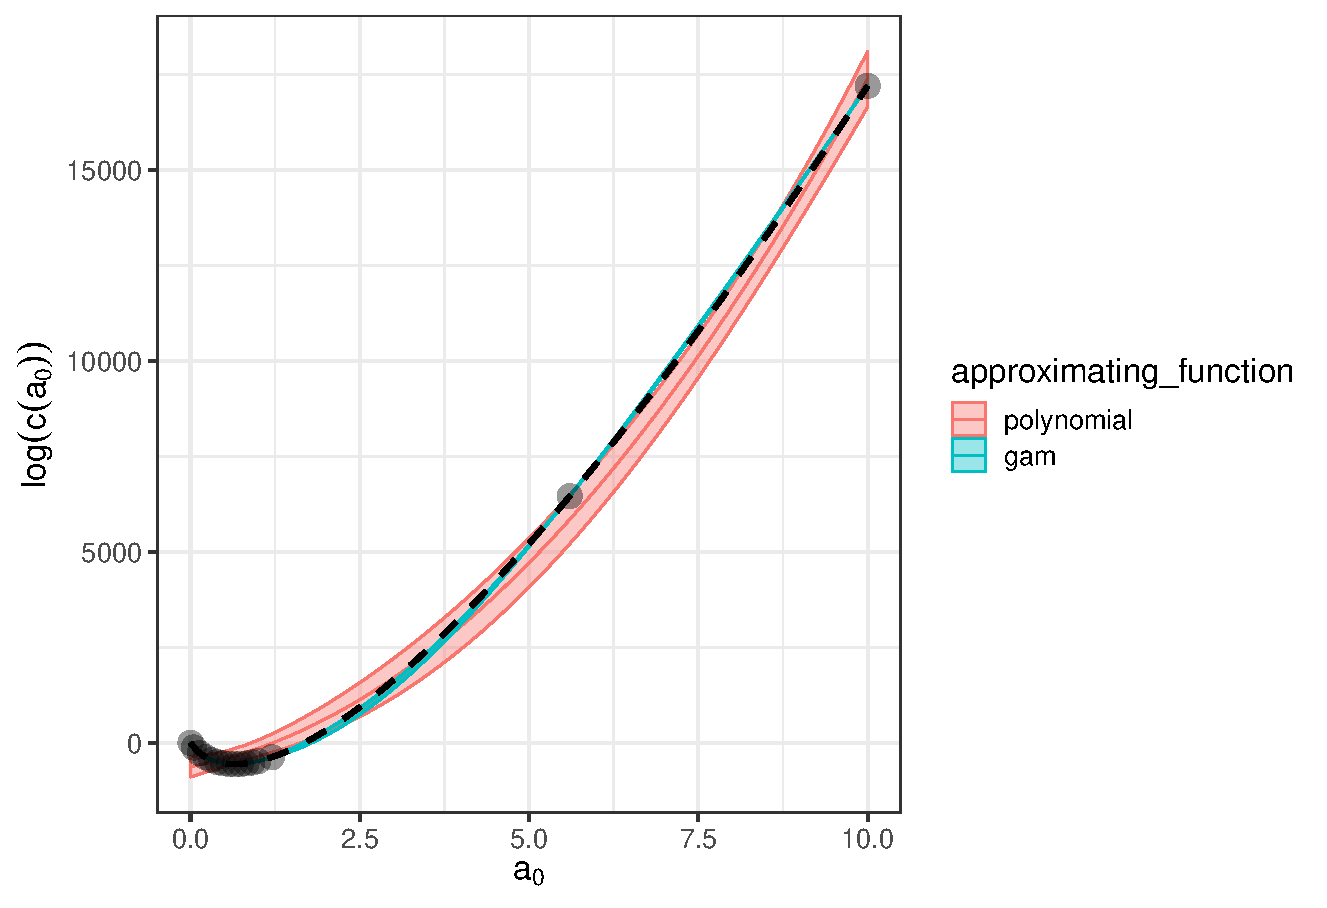
\includegraphics[width=7cm]{../figures/estimates_log_ca0_Gaussian.pdf}}
\hfill
\subfigure[Inverse-Gaussian]{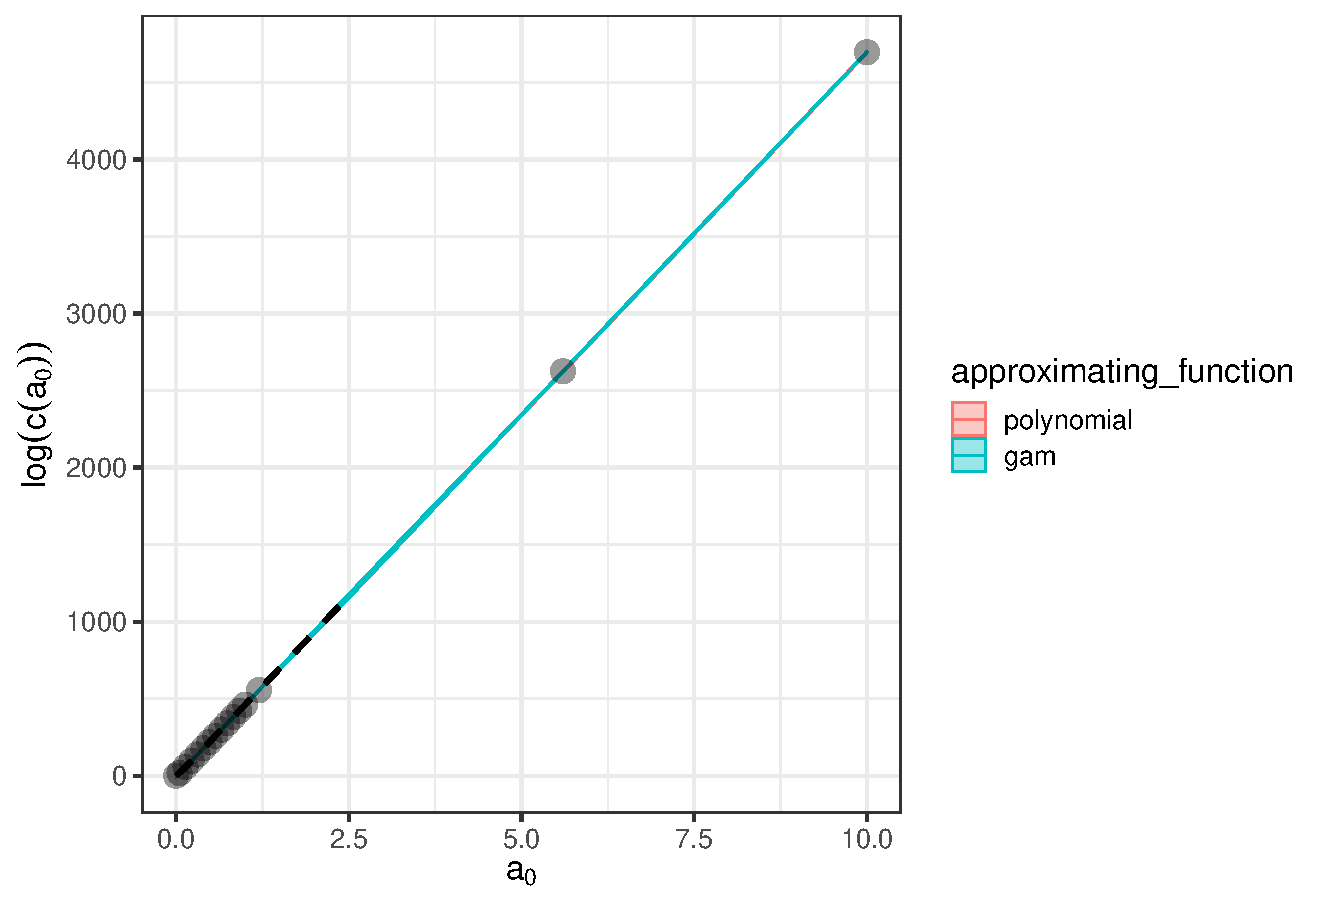
\includegraphics[width=7cm]{../figures/estimates_log_ca0_invGaussian.pdf}}\\
\hfill
\subfigure[Linear regression]{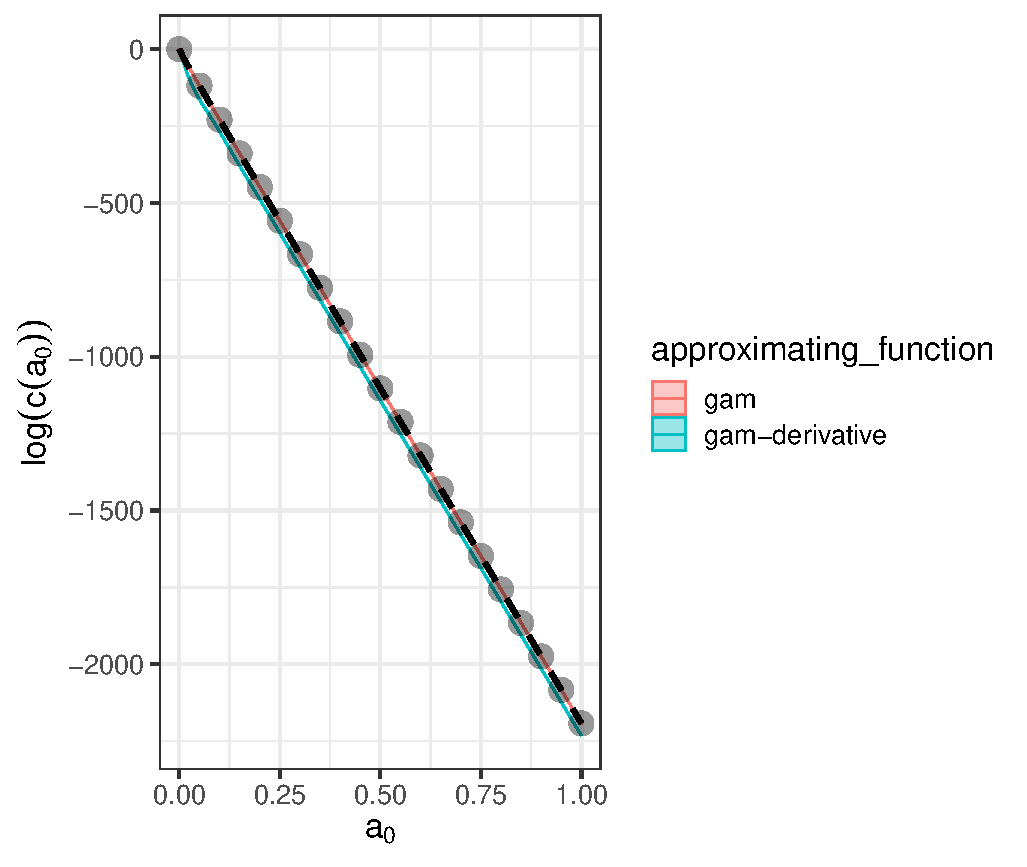
\includegraphics[width=7cm]{../figures/estimates_log_ca0_RegressionNIG.pdf}}
\hfill
\subfigure[Logistic regression]{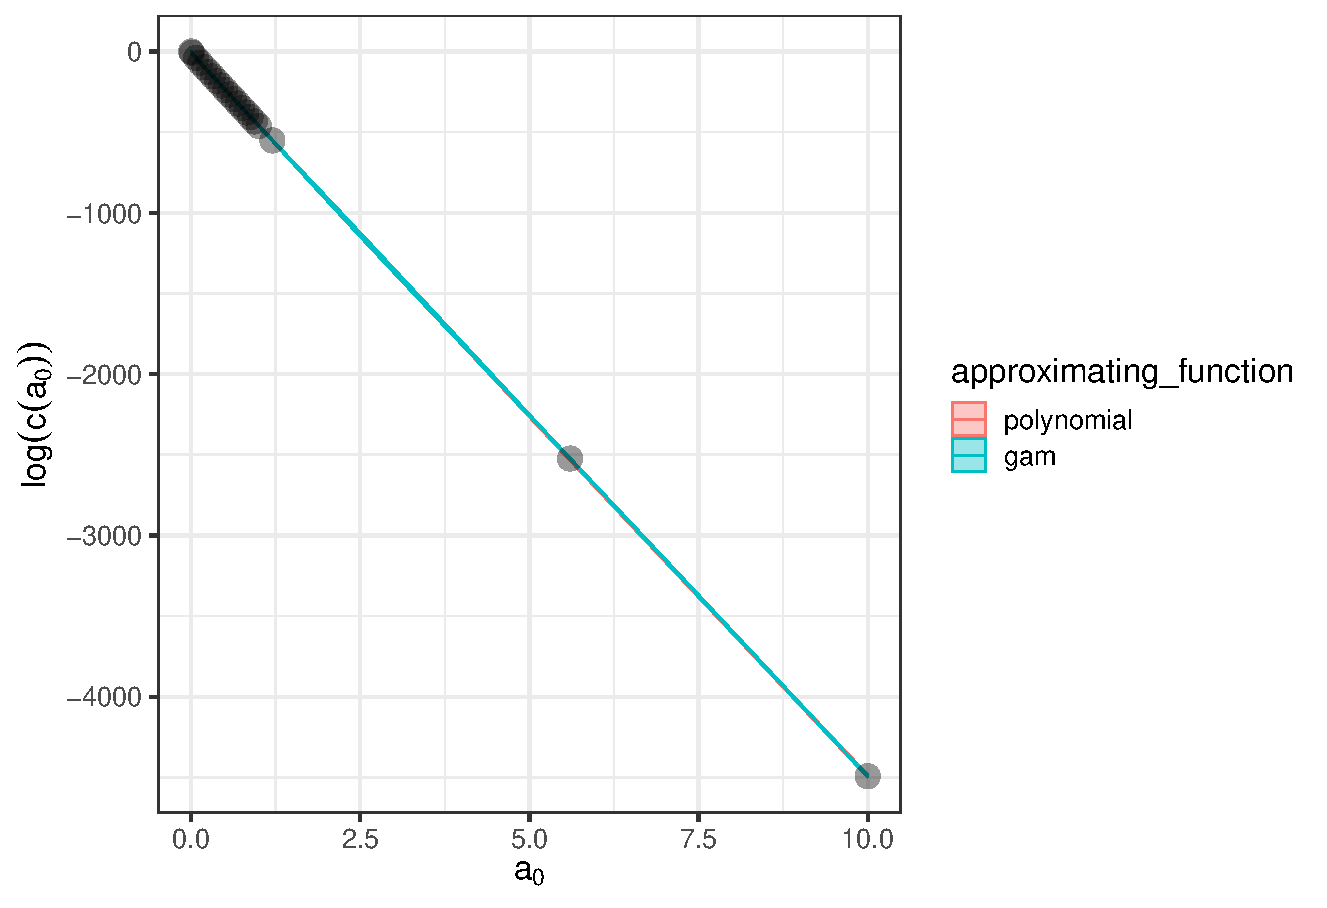
\includegraphics[width=7cm]{../figures/estimates_log_ca0_RegressionLogistic.pdf}}

\caption{\textbf{The normalising constant $c(a_0)$ for several models}.
The plots show $\log c(a_0)$ for a host of models.
Notice how for the inverse-Gaussian model  $\log c(a_0)$ is~\textbf{increasing} in $a_0$.
Dashed line shows the true $c(a_0)$, when it exists or can be computed.
}
\label{fig:cA0}
\end{figure}

\begin{figure}
\hfill
\subfigure[Gaussian]{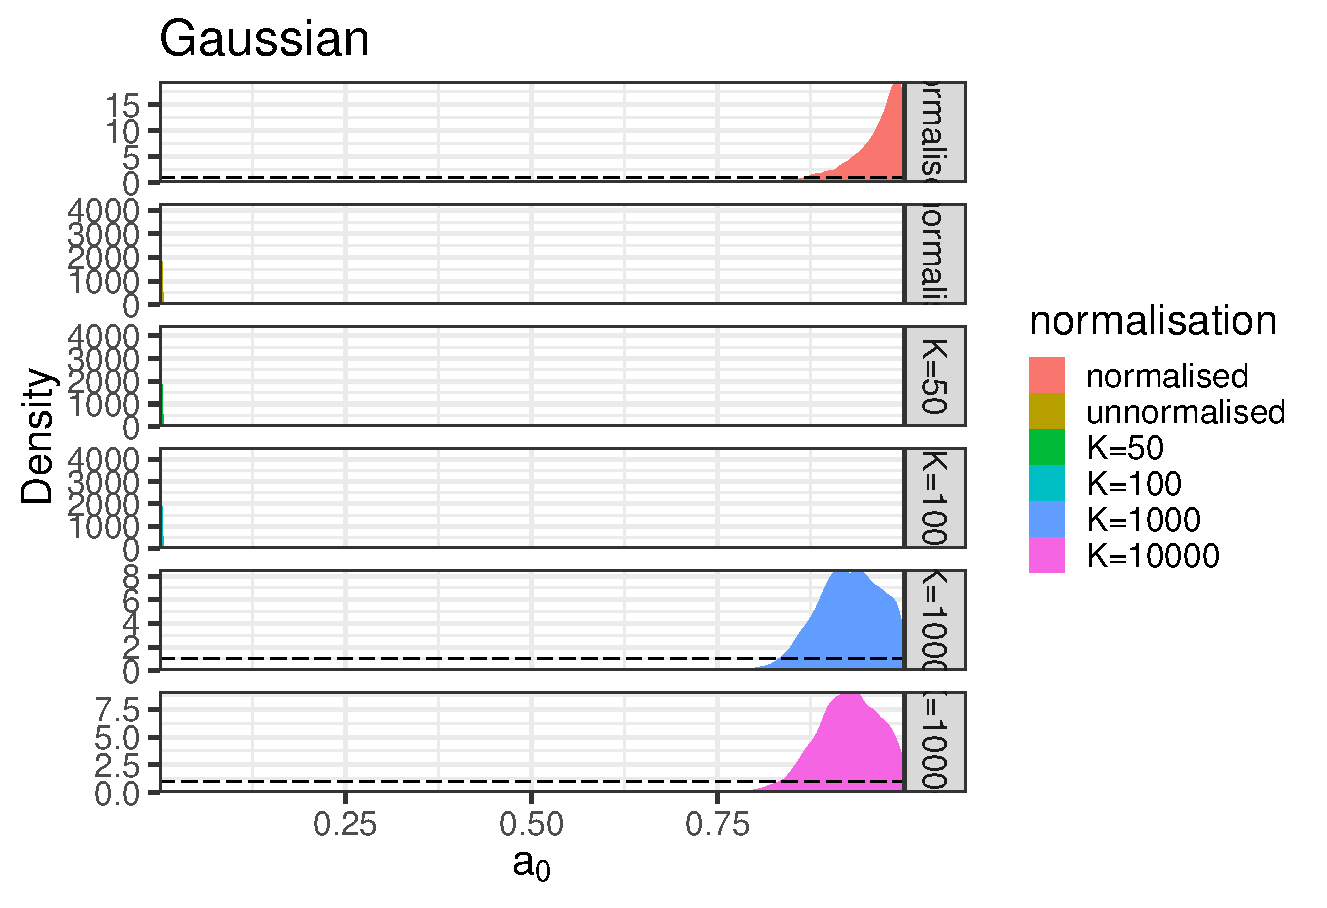
\includegraphics[width=7cm]{../figures/a0_posterior_Gaussian.pdf}}
\hfill
\subfigure[Inverse-Gaussian]{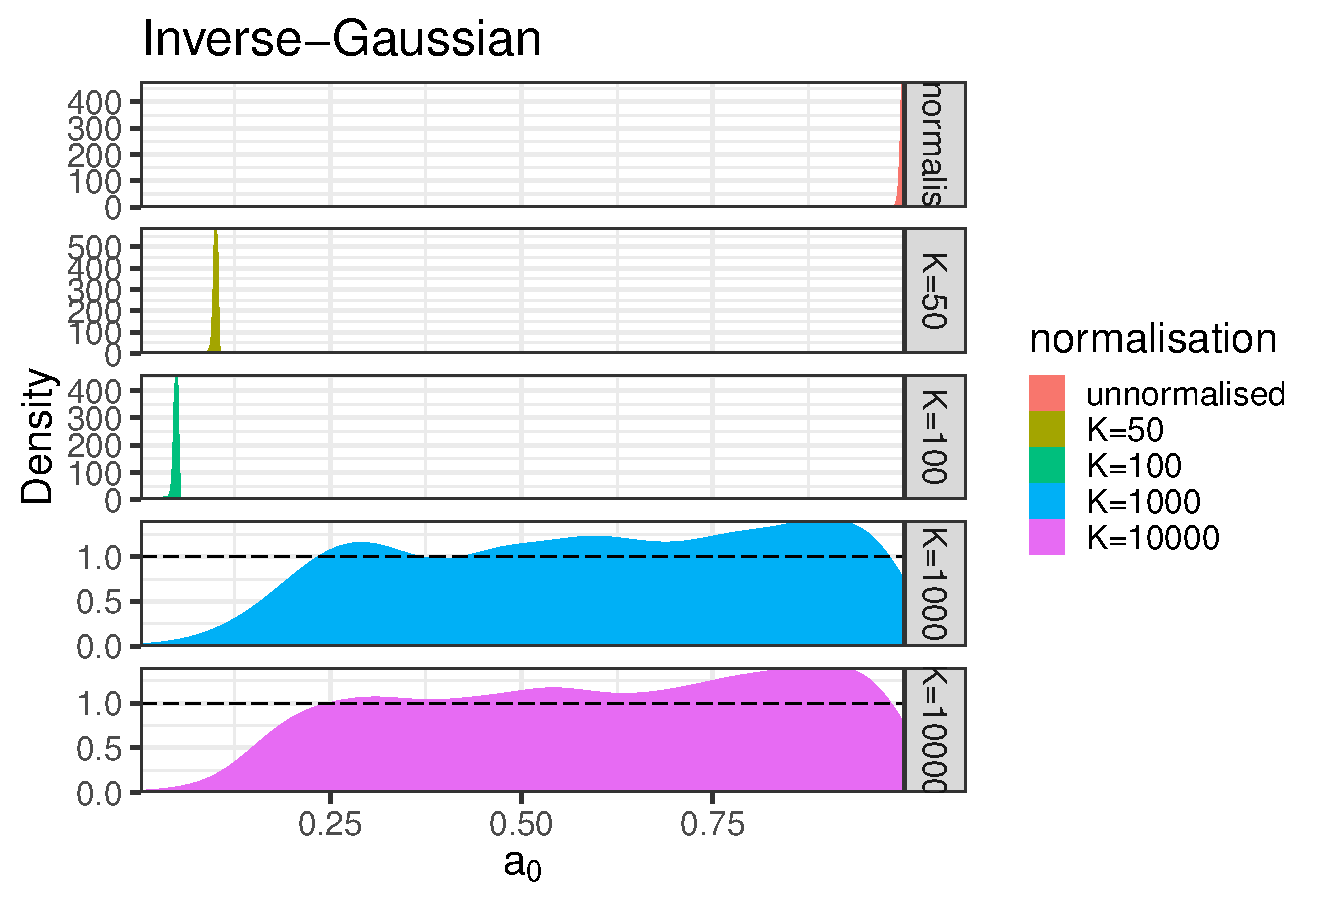
\includegraphics[width=7cm]{../figures/a0_posterior_invgaussian.pdf}}\\
\hfill
\subfigure[Linear regression]{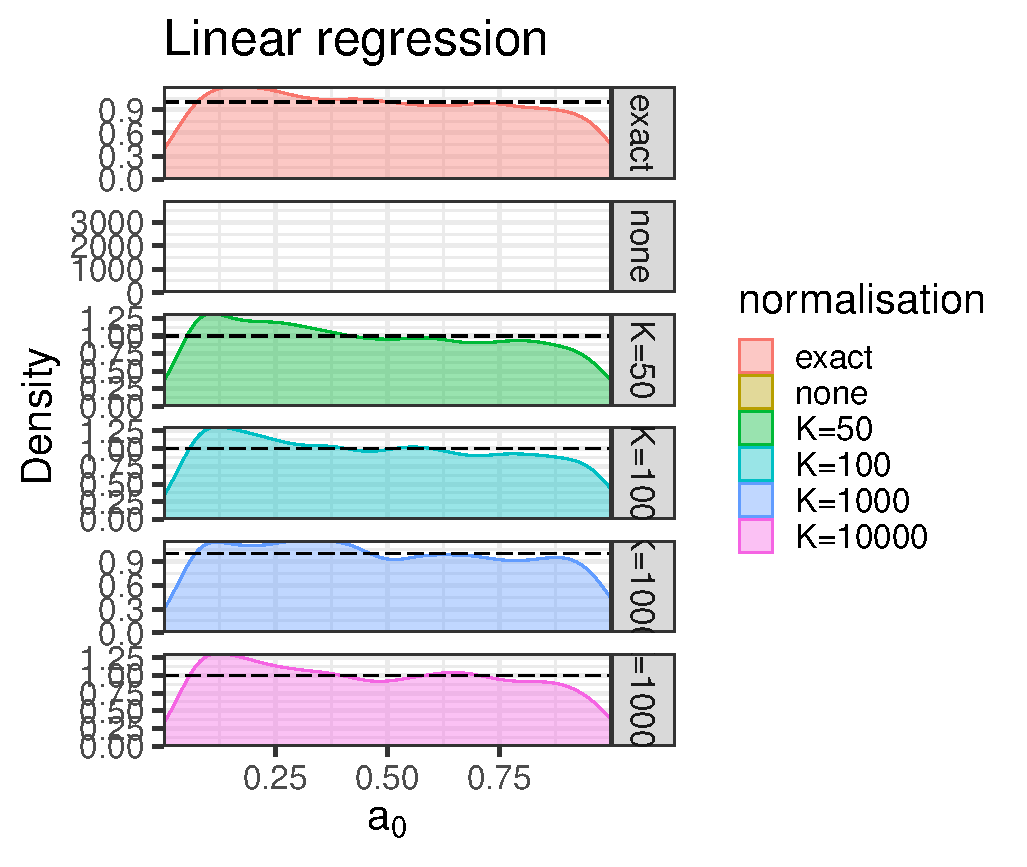
\includegraphics[width=7cm]{../figures/a0_posterior_RegressionNIG.pdf}}
\hfill
\subfigure[Logistic regression]{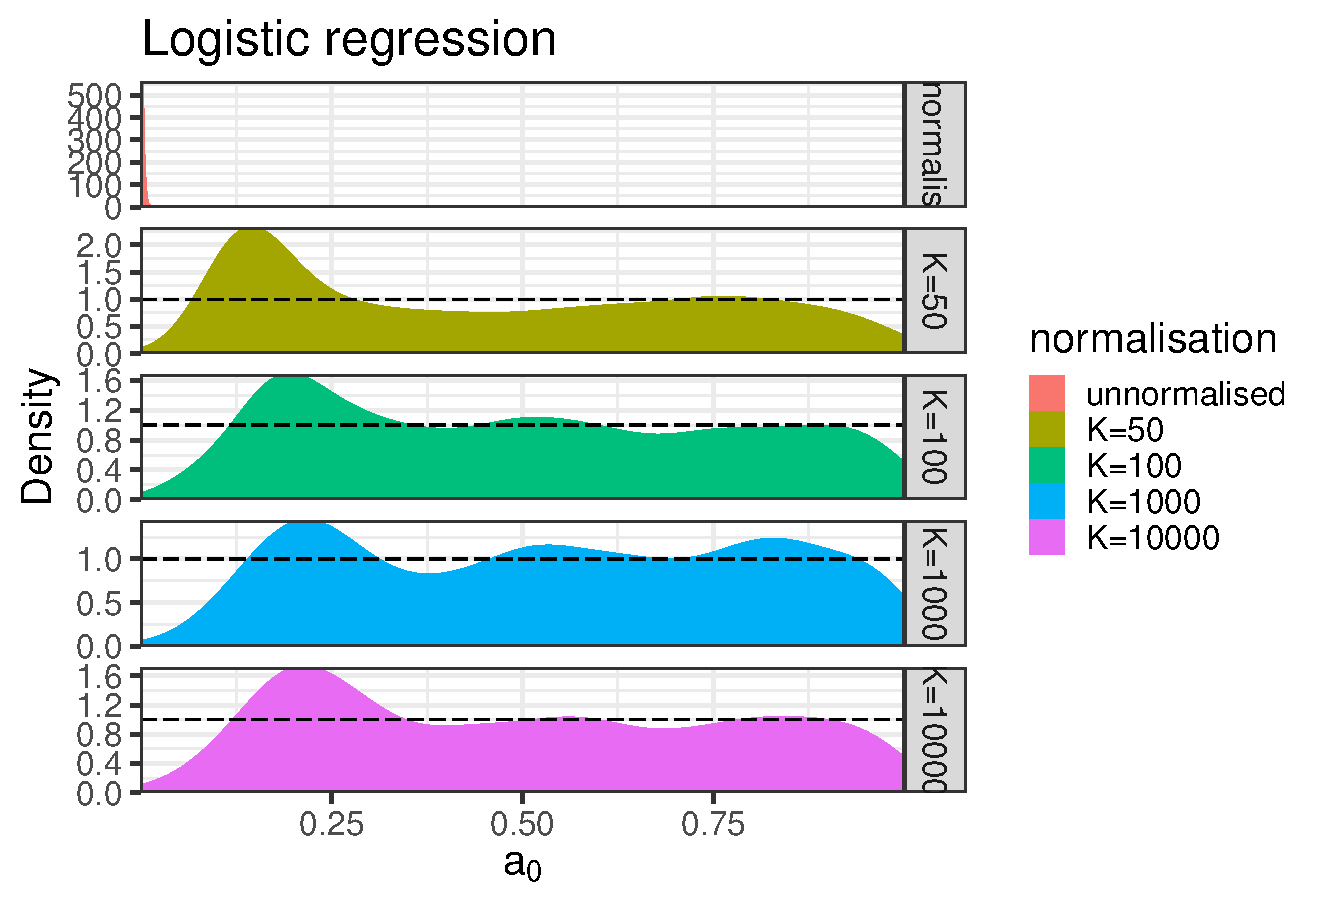
\includegraphics[width=7cm]{../figures/a0_posterior_RegressionLogistic.pdf}}
\hfill
\caption{\textbf{The posterior distribution of $a_0$ under normalised and unnormalised models}.
The panels (and colours) correspond to the posterior distribution of the parameter $a_0$ when $c(a_0)$ is accounted for and when it is not included.
Horizontal dashed lines show the prior density of a $\text{Beta}(\nu = 1, \eta = 1)$.
}
\label{fig:normalisation}
\end{figure}

\begin{figure}
\hfill
\subfigure[Gaussian]{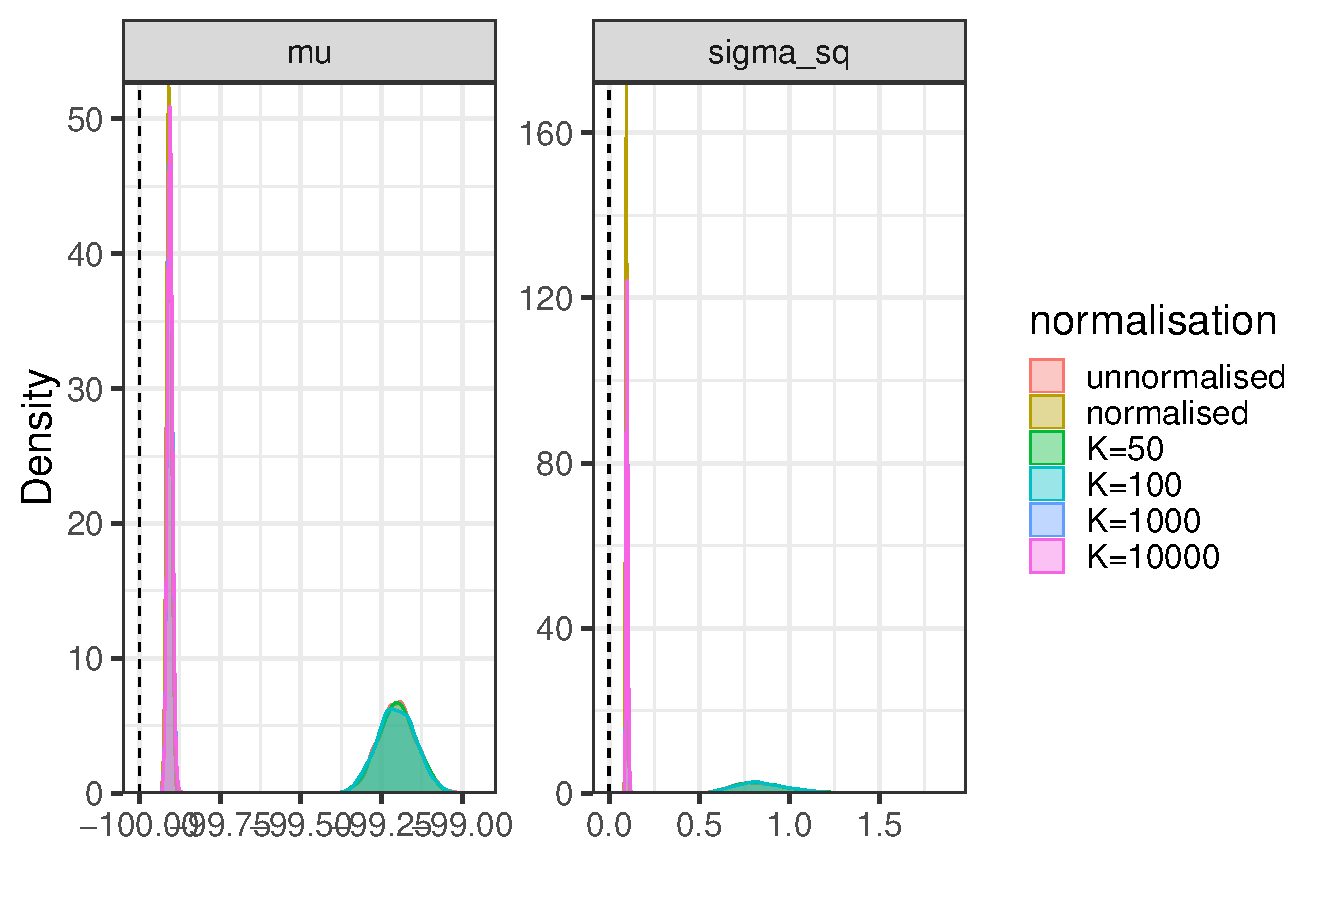
\includegraphics[width=7cm]{../figures/parameter_posterior_Gaussian.pdf}}
\hfill
\subfigure[Inverse-Gaussian]{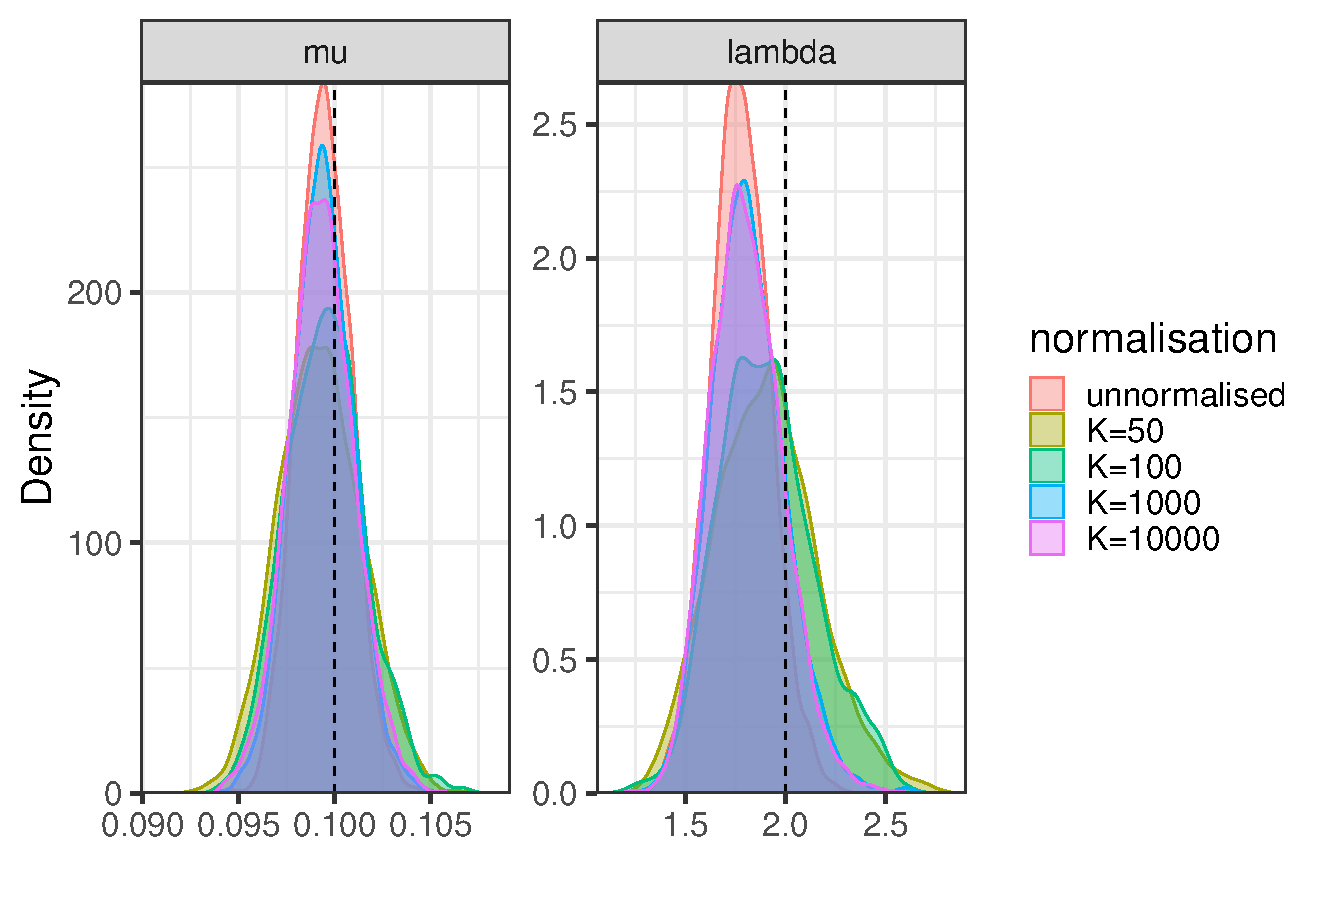
\includegraphics[width=7cm]{../figures/parameter_posterior_invgaussian.pdf}}\\
\hfill
\subfigure[Linear regression]{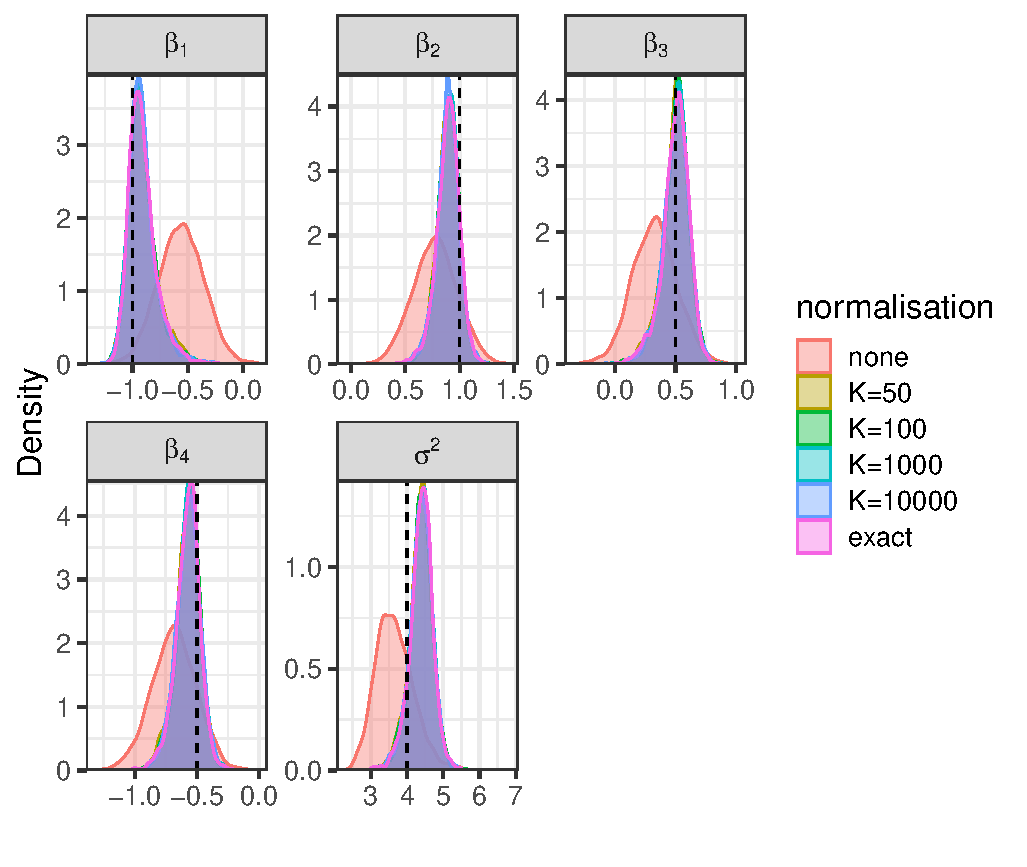
\includegraphics[width=7cm]{../figures/parameter_posterior_Regression.pdf}}
\hfill
\subfigure[Logistic regression]{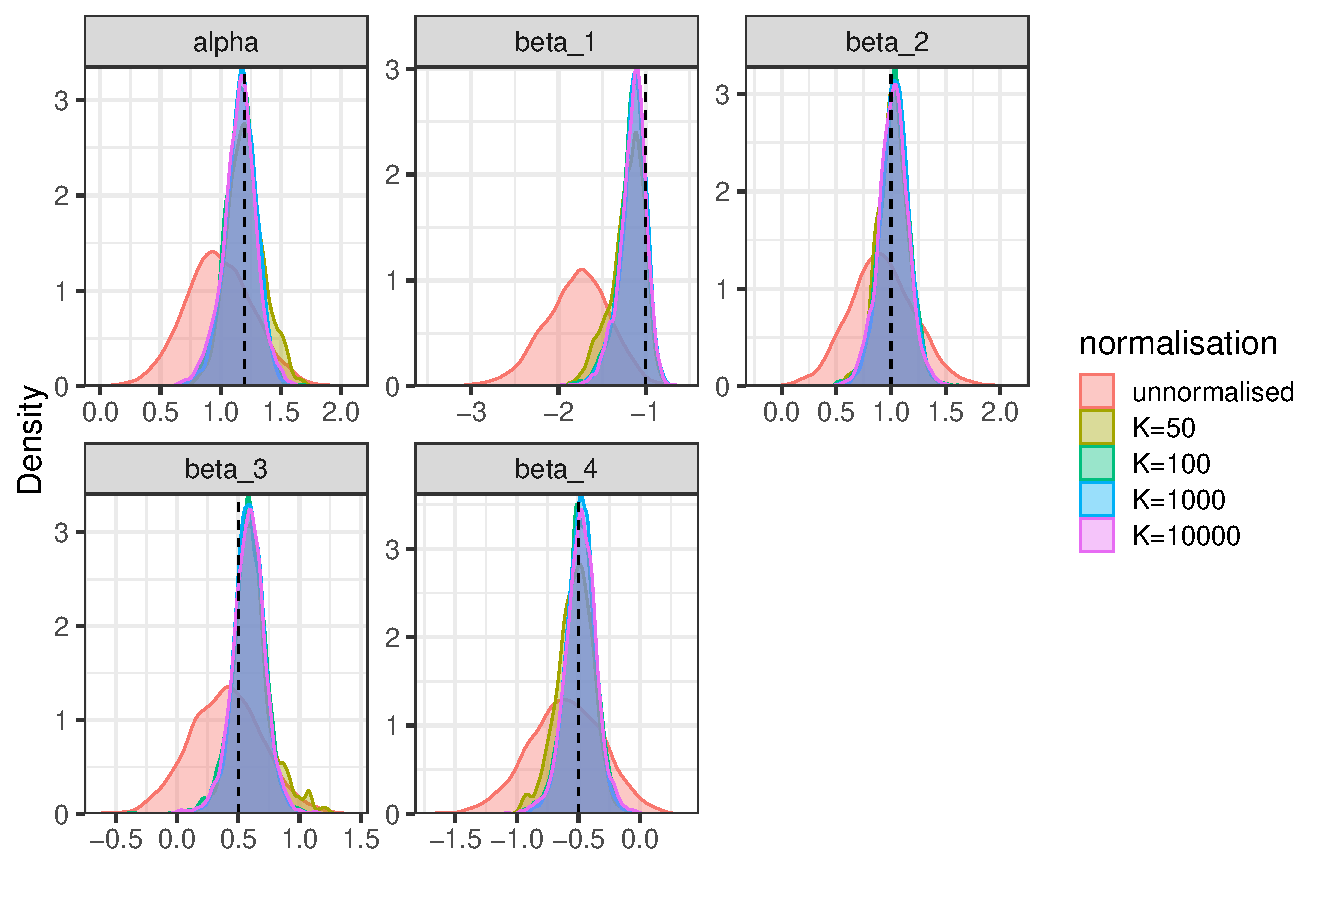
\includegraphics[width=7cm]{../figures/parameter_posterior_LogisticRegression.pdf}}
\hfill
\caption{\textbf{The posterior distribution of parameters of interest under normalised and unnormalised models}.
The panels (and colours) correspond to the posterior distribution of the parameter $a_0$ when $c(a_0)$ is accounted for and when it is not included.
Vertical lines mark the data-generating parameter values.
}
\label{fig:parameter_estimates}
\end{figure}
\end{document}
